\documentclass[12pt, titlepage]{article}

\usepackage{fullpage}
\usepackage[round]{natbib}
\usepackage{multirow}
\usepackage{booktabs}
\usepackage{tabularx}
\usepackage{graphicx}
\usepackage{float}
\usepackage{hyperref}
\hypersetup{
    colorlinks,
    citecolor=blue,
    filecolor=black,
    linkcolor=red,
    urlcolor=blue
}

%% Comments

\usepackage{color}

\newif\ifcomments\commentstrue %displays comments
%\newif\ifcomments\commentsfalse %so that comments do not display

\ifcomments
\newcommand{\authornote}[3]{\textcolor{#1}{[#3 ---#2]}}
\newcommand{\todo}[1]{\textcolor{red}{[TODO: #1]}}
\else
\newcommand{\authornote}[3]{}
\newcommand{\todo}[1]{}
\fi

\newcommand{\wss}[1]{\authornote{blue}{SS}{#1}} 
\newcommand{\plt}[1]{\authornote{magenta}{TPLT}{#1}} %For explanation of the template
\newcommand{\an}[1]{\authornote{cyan}{Author}{#1}}

%% Common Parts

\newcommand{\progname}{Housemates} % PUT YOUR PROGRAM NAME HERE
\newcommand{\authname}{Team \#9, Housemates
\\ Justin Dang - dangj15 
\\ Harris Hamid - hamidh1
\\ Fady Morcos - morcof2 
\\ Rizwan Ahsan - ahsanm7
\\ Sheikh Afsar - afsars} % AUTHOR NAMES                  

\usepackage{hyperref}
    \hypersetup{colorlinks=true, linkcolor=blue, citecolor=blue, filecolor=blue,
                urlcolor=blue, unicode=false}
    \urlstyle{same}
                                


\newcounter{acnum}
\newcommand{\actheacnum}{AC\theacnum}
\newcommand{\acref}[1]{AC\ref{#1}}

\newcounter{ucnum}
\newcommand{\uctheucnum}{UC\theucnum}
\newcommand{\uref}[1]{UC\ref{#1}}

\newcounter{mnum}
\newcommand{\mthemnum}{M\themnum}
\newcommand{\mref}[1]{M\ref{#1}}

\begin{document}

\title{Module Guide for \progname{}} 
\author{\authname}
\date{\today}

\maketitle

\pagenumbering{roman}

\section{Revision History}

\begin{tabularx}{\textwidth}{p{3cm}p{2cm}X}
\toprule {\bf Date} & {\bf Version} & {\bf Notes}\\
\midrule
January 17, 2024 & 1.0 & Revision 0\\
April 03, 2024 & 2.0 & Revision 1\\
\bottomrule
\end{tabularx}

\newpage

\section{Reference Material}

This section records information for easy reference.

\subsection{Abbreviations and Acronyms}

\renewcommand{\arraystretch}{1.2}
\begin{tabular}{l l} 
  \toprule		
  \textbf{symbol} & \textbf{description}\\
  \midrule 
  AC & Anticipated Change\\
  DAG & Directed Acyclic Graph \\
  M & Module \\
  MG & Module Guide \\
  OS & Operating System \\
  R & Requirement\\
  SRS & Software Requirements Specification\\
  Housemates & Explanation of program name\\
  UC & Unlikely Change \\
  \bottomrule
\end{tabular}\\

\newpage

\tableofcontents

\listoftables

\listoffigures

\newpage

\pagenumbering{arabic}

\section{Introduction}

Decomposing a system into modules is a commonly accepted approach to developing
software.  A module is a work assignment for a programmer or programming
team~\citep{ParnasEtAl1984}.  We advocate a decomposition
based on the principle of information hiding~\citep{Parnas1972a}.  This
principle supports design for change, because the ``secrets'' that each module
hides represent likely future changes.  Design for change is valuable in SC,
where modifications are frequent, especially during initial development as the
solution space is explored.  

Our design follows the rules layed out by \citet{ParnasEtAl1984}, as follows:
\begin{itemize}
\item System details that are likely to change independently should be the
  secrets of separate modules.
\item Each data structure is implemented in only one module.
\item Any other program that requires information stored in a module's data
  structures must obtain it by calling access programs belonging to that module.
\end{itemize}

After completing the first stage of the design, the Software Requirements
Specification (SRS), the Module Guide (MG) is developed~\citep{ParnasEtAl1984}. The MG
specifies the modular structure of the system and is intended to allow both
designers and maintainers to easily identify the parts of the software.  The
potential readers of this document are as follows:

\begin{itemize}
\item New project members: This document can be a guide for a new project member
  to easily understand the overall structure and quickly find the
  relevant modules they are searching for.
\item Maintainers: The hierarchical structure of the module guide improves the
  maintainers' understanding when they need to make changes to the system. It is
  important for a maintainer to update the relevant sections of the document
  after changes have been made.
\item Designers: Once the module guide has been written, it can be used to
  check for consistency, feasibility, and flexibility. Designers can verify the
  system in various ways, such as consistency among modules, feasibility of the
  decomposition, and flexibility of the design.
\end{itemize}

The rest of the document is organized as follows. Section
\ref{SecChange} lists the anticipated and unlikely changes of the software
requirements. Section \ref{SecMH} summarizes the module decomposition that
was constructed according to the likely changes. Section \ref{SecConnection}
specifies the connections between the software requirements and the
modules. Section \ref{SecMD} gives a detailed description of the
modules. Section \ref{SecTM} includes two traceability matrices. One checks
the completeness of the design against the requirements provided in the SRS. The
other shows the relation between anticipated changes and the modules. Section
\ref{SecUse} describes the use relation between modules.  Section \ref{Timeline} describes the timeline to complete revision 0 of \progname{}. Section \ref{Reflection} contains the reflection for the design stage of \progname{}.

\section{Anticipated and Unlikely Changes} \label{SecChange}

This section lists possible changes to the system. According to the likeliness
of the change, the possible changes are classified into two
categories. Anticipated changes are listed in Section \ref{SecAchange}, and
unlikely changes are listed in Section \ref{SecUchange}.

\subsection{Anticipated Changes} \label{SecAchange}

Anticipated changes are the source of the information that is to be hidden
inside the modules. Ideally, changing one of the anticipated changes will only
require changing the one module that hides the associated decision. The approach
adapted here is called design for
change.

\begin{description}
\item[\refstepcounter{acnum} \actheacnum \label{acHardware}:] The specific
  hardware on which the software is running.
\item[\refstepcounter{acnum} \actheacnum \label{acInput}:] The format of the initial input data.
\item[\refstepcounter{acnum} \actheacnum \label{acAccount}:] The algorithms used for account verification.
\item[\refstepcounter{acnum} \actheacnum \label{acBillManagement}:] The algorithms used to determine how bills are split between users.
\item[\refstepcounter{acnum} \actheacnum \label{acTaskManagement}:] The algorithms used in the task management system.
\item[\refstepcounter{acnum} \actheacnum \label{acScheduling}:] The algorithms used in the scheduling system.
\end{description}

\subsection{Unlikely Changes} \label{SecUchange}

The module design should be as general as possible. However, a general system is more complex. Sometimes this complexity is not necessary. Fixing some design
decisions at the system architecture stage can simplify the software design. If these decision should later need to be changed, then many parts of the design will potentially need to be modified. Hence, it is not intended that these decisions will be changed.

\begin{description}
\item[\refstepcounter{ucnum} \uctheucnum \label{ucIO}:] Inputting data requires mouse or touch screen, output data are displayed to the device screen
\item[\refstepcounter{ucnum} \uctheucnum \label{ucDatabase}:] The database will be MongoDB
\item[\refstepcounter{ucnum} \uctheucnum \label{ucNetwork}:] Changes in the network libraries used.
\item[\refstepcounter{ucnum} \uctheucnum \label{ucServer}:] The server will run on NodeJS
\end{description}

\section{Module Hierarchy} \label{SecMH}

This section provides an overview of the module design. Modules are summarized
in a hierarchy decomposed by secrets in Table \ref{TblMH}. The modules listed
below, which are leaves in the hierarchy tree, are the modules that will
actually be implemented.

\begin{description}
\item [\refstepcounter{mnum} \mthemnum \label{mHH}:] Hardware-Hiding Module
\item [\refstepcounter{mnum} \mthemnum \label{mT}:] Task Management Module
\item [\refstepcounter{mnum} \mthemnum \label{mB}:] Bill Management Module
\item [\refstepcounter{mnum} \mthemnum \label{mS}:] Scheduling Module
\item [\refstepcounter{mnum} \mthemnum \label{mA}:] Account Module
\item [\refstepcounter{mnum} \mthemnum \label{mDM}:] Database Model
\item [\refstepcounter{mnum} \mthemnum \label{mD}:] Database Driver Module
\end{description}


\begin{table}[h!]
\centering
\begin{tabular}{p{0.3\textwidth} p{0.6\textwidth}}
\toprule
\textbf{Level 1} & \textbf{Level 2}\\
\midrule

{Hardware-Hiding Module} & ~ \\
\midrule

\multirow{5}{0.3\textwidth}{Behaviour-Hiding Module} 
& Task Management Module\\
& Bill Management Module\\
& Scheduling Module\\
& Account Module\\
& Database Model\\
\midrule

{Software Decision Module}
& Database Driver Module\\
\bottomrule

\end{tabular}
\caption{Module Hierarchy}
\label{TblMH}
\end{table}

\section{Connection Between Requirements and Design} \label{SecConnection}

The design of the system is intended to satisfy the requirements developed in
the SRS. In this stage, the system is decomposed into modules. The connection
between requirements and modules is listed in Table~\ref{TblRT}.

\section{Module Decomposition} \label{SecMD}

Modules are decomposed according to the principle of ``information hiding''
proposed by \citet{ParnasEtAl1984}. The \emph{Secrets} field in a module
decomposition is a brief statement of the design decision hidden by the
module. The \emph{Services} field specifies \emph{what} the module will do
without documenting \emph{how} to do it. For each module, a suggestion for the
implementing software is given under the \emph{Implemented By} title. If the
entry is \emph{OS}, this means that the module is provided by the operating
system or by standard programming language libraries.  \emph{\progname{}} means the
module will be implemented by the \progname{} software.

Only the leaf modules in the hierarchy have to be implemented. If a dash
(\emph{--}) is shown, this means that the module is not a leaf and will not have
to be implemented.

\subsection{Hardware Hiding Modules (\mref{mHH})}

\begin{description}
\item[Secrets:]The data structure and algorithm used to implement the virtual
  hardware.
\item[Services:]Serves as a virtual hardware used by the rest of the
  system. This module provides the interface between the hardware and the
  software. So, the system can use it to display outputs or to accept inputs.
\item[Implemented By:] OS
\end{description}

\subsection{Behaviour-Hiding Module}

\begin{description}
\item[Secrets:]The contents of the required behaviours.
\item[Services:]Includes programs that provide externally visible behaviour of
  the system as specified in the software requirements specification (SRS)
  documents. This module serves as a communication layer between the
  hardware-hiding module and the software decision module. The programs in this
  module will need to change if there are changes in the SRS.
\item[Implemented By:] --
\end{description}


\subsubsection{Task Management Module (\mref{mT})}

\begin{description}
\item[Secrets:]The format and structure of the input data. The algorithms used for the task management functionality.
\item[Services:] Provides the task management functionality of the application. Converts the input data into the data structure used by the database interface module. 
\item[Implemented By:] \progname{}
\item[Type of Module:] Library
\end{description}


\subsubsection{Bill Management Module (\mref{mB})}

\begin{description}
\item[Secrets:]The format and structure of the input data. The algorithms used for the bill splitting functionality.
\item[Services:] Provides the bill management and bill splitting functionality of the application. Converts the input data into the data structure used by the database interface module. 
\item[Implemented By:] \progname{}
\item[Type of Module:] Library
\end{description}

\subsubsection{Scheduling Module (\mref{mS})}

\begin{description}
\item[Secrets:] The format and structure of the input data. The algorithms used for the scheduling functionality.
\item[Services:] Provides the scheduling functionality of the application. Converts the input data into the data structure used by the database interface module. 
\item[Implemented By:] \progname{}
\item[Type of Module:] Library
\end{description}

\subsubsection{Account Module (\mref{mA})}

\begin{description}
\item[Secrets:] The format and structure of the input data. The algorithms used for the account verification.
\item[Services:] Provides the account functionality of the application. Converts the input data into the data structure used by the database interface module. 
\item[Implemented By:] \progname{}
\item[Type of Module:] Library
\end{description}

\subsubsection{Database Model (\mref{mDM})}

\begin{description}
\item[Secrets:] The data structures for representing the database schema
\item[Services:] Provides data to be inputted into the database using the same schema defined.
\item[Implemented By:] \progname{}
\item[Type of Module:] Library
\end{description}

\subsection{Software Decision Module}

\begin{description}
\item[Secrets:] The design decision based on mathematical theorems, physical
  facts, or programming considerations. The secrets of this module are
  \emph{not} described in the SRS.
\item[Services:] Includes data structure and algorithms used in the system that
  do not provide direct interaction with the user. 
  % Changes in these modules are more likely to be motivated by a desire to
  % improve performance than by externally imposed changes.
\item[Implemented By:] --
\end{description}

\subsubsection{Database Driver Module (\mref{mD})}
\begin{description}
\item[Secrets:] The specific details of making changes to the data in the database.
\item[Services:] Facilitates communication between the database and the other modules.
\item[Implemented By:] \progname{}, MongoDB
\item[Type of Module:] Library
\end{description}

\section{Traceability Matrix} \label{SecTM}

This section shows two traceability matrices: between the modules and the requirements as seen in \citep{SRS} and between the modules and the anticipated changes.

% the table should use mref, the requirements should be named, use something
% like fref
\begin{table}[H]
\centering
\begin{tabular}{p{0.2\textwidth} p{0.6\textwidth}}
\toprule
\textbf{Req.} & \textbf{Modules}\\
\midrule
TM1-5 & \mref{mT}\\
BM1-7 & \mref{mB}\\
SS1-3 & \mref{mS}\\
AS1-5 & \mref{mA}\\
LF-A1 & \mref{mT}, \mref{mB}, \mref{mS}, \mref{mA}\\
UH-E1 & \mref{mT}, \mref{mB}, \mref{mS}, \mref{mA}\\
UH-P1 & \mref{mT}, \mref{mB}, \mref{mS}, \mref{mA}\\
UH-L1 & \mref{mT}, \mref{mB}, \mref{mS}, \mref{mA}\\
UH-A1 & \mref{mT}, \mref{mB}, \mref{mS}, \mref{mA}\\
P-SL1 & \mref{mT}, \mref{mB}, \mref{mS}, \mref{mA}, \mref{mD}\\
P-PA1 & \mref{mB}\\
P-RFT1 & \mref{mT}, \mref{mB}, \mref{mS}, \mref{mA}, \mref{mD}\\
P-C1 & \mref{mT}, \mref{mB}, \mref{mS}, \mref{mA}, \mref{mD}\\
OE-PE1 & \mref{mHH}\\
S-A1 & \mref{mT}, \mref{mB}, \mref{mS}, \mref{mA}\\
S-IN1 & \mref{mT}, \mref{mB}, \mref{mS}, \mref{mA}, \mref{mDM}, \mref{mD}\\
S-P1 & \mref{mA}, \mref{mD}\\
\bottomrule
\end{tabular}
\caption{Trace Between Requirements and Modules}
\label{TblRT}
\end{table}

\begin{table}[H]
\centering
\begin{tabular}{p{0.2\textwidth} p{0.6\textwidth}}
\toprule
\textbf{AC} & \textbf{Modules}\\
\midrule
\acref{acHardware} & \mref{mHH}\\
\acref{acInput} & \mref{mT}, \mref{mB}, \mref{mS}, \mref{mA}, \mref{mDM}\\
\acref{acAccount} & \mref{mA}\\
\acref{acBillManagement} & \mref{mB}\\
\acref{acTaskManagement} & \mref{mT}\\
\acref{acScheduling} & \mref{mS}\\
\bottomrule
\end{tabular}
\caption{Trace Between Anticipated Changes and Modules}
\label{TblACT}
\end{table}

\section{Use Hierarchy Between Modules} \label{SecUse}

In this section, the uses hierarchy between modules is
provided. \citet{Parnas1978} said of two programs A and B that A {\em uses} B if correct execution of B may be necessary for A to complete the task described in its specification. That is, A {\em uses} B if there exist situations in which the correct functioning of A depends upon the availability of a correct implementation of B.  Figure \ref{FigUH} illustrates the use relation between the modules. It can be seen that the graph is a directed acyclic graph (DAG). Each level of the hierarchy offers a testable and usable subset of the system, and modules in the higher level of the hierarchy are essentially simpler
because they use modules from the lower levels.

\begin{figure}[H]
\centering
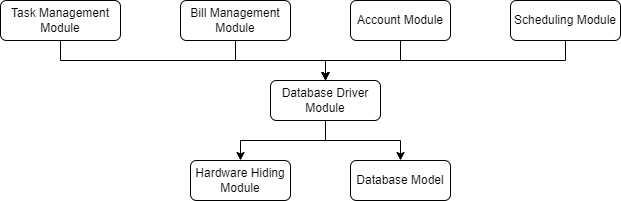
\includegraphics[width=\textwidth]{UsesHierarchy.png}
\caption{Use hierarchy among modules}
\label{FigUH}
\end{figure}


\section{Timeline for Revision 0} \label{Timeline}

\begin{table}[H]
    \centering
    \begin{tabular}{|>{\raggedright}p{0.2\textwidth}|p{0.4\textwidth}|p{0.125\textwidth}|p{0.2\textwidth}|}
    \hline
    \textbf{Modules} & \textbf{Rev 0 Implementation Tasks} & \textbf{Deadline} & \textbf{Team Members Responsible}\\
    \hline
     Hardware-Hiding Module & Provided by OS & N/A & N/A\\
    \hline
     Task Management Module & Implement all the functions included in the module & February 4, 2024 & Justin, Harris\\
    \hline
    Bill Management Module & Implement all the functions included in the module & February 4, 2024 & Harris, Fardeen\\
    \hline
    Scheduling Module & Implement all the functions included in the module & February 4, 2024 & Rizwan, Fady\\
    \hline
    Account Module & Implement all the functions included in the module & February 1, 2024 & Fardeen, Rizwan\\
    \hline
    Interface Design Module & Implement all the functions included in the module & February 4, 2024 & Fady, Justin\\
    \hline
    Database Interface  Module & Set up MongoDB Schema and Mongoose objects & February 1, 2024 & Fardeen, Rizwan\\
    \hline
    Testing and Verification & Unit testing of functions in modules & February 6, 2024 & Everyone\\
    \hline
     Network Interface Module & Set up API Routes as required & February 4, 2024 & Everyone\\
    \hline
     Cryptography Module & Provided by external libraries & N/A & N/A\\
    \hline
    \end{tabular}
    \caption{Timeline}
    \label{tab:timeline}
\end{table}

Though team members are designated to specific modules and tasks, it's crucial to understand that this doesn't create rigid boundaries. The assignments highlight primary responsibilities and leadership roles in developing particular components. While certain individuals lead the charge for specific modules, all team members actively contribute, albeit with varying degrees of impact. The designated leads play a central role in shaping the direction of development for their respective areas, encouraging a collaborative approach within the team.


\section{Reflection} \label{Reflection}

The information in this section will be used to evaluate the team members on the graduate attribute of Problem Analysis and Design.  Please answer the following questions:

\begin{enumerate}
  \item \textbf{What are the limitations of your solution?  Put another way, given unlimited resources, what could you do to make the project better? (LO\_ProbSolutions)}
  \\
  \\
  The main limitations of the Housemates application right now is the lack of integration that Housemates has with other software at the current moment. For example, the scheduling feature of the Housemates application could be integrated with popular calendar services like Google calendar. Many features had to be scoped down to meet the time constraint we had and many other features had to be cut together. Some of the features and ideas we had discussed are:
  \begin{itemize}
      \item Implementing a way to attach pictures or pdf to bills and tasks
      \item Adding natural language processing (NLP) in our application e.g. add receipt picture to automatically add the bill, same for tasks
      \item Further optimizations in terms of performance
      \item More emphasis and support for accessibility settings
  \end{itemize}
  We believe these features would be nice to include in our application and would greatly improve its quality, however many of them are not feasible given the limited development time frame we have.
  \\
  \\
  Additionally, monetary limitations have led to further constraints on the development of our application.
  Given unlimited money, improvements could be made to our database and server. In particular,
  a greater capacity database and higher bandwidth server would have been nice in terms of scalability of our
  project. With the additional funds, we would be able to create an application that better aligns with our goal
  by allowing more users to use the application.
  \\
  \item \textbf{Give a brief overview of other design solutions you considered.  What are the benefits and tradeoffs of those other designs compared with the chosen design?  From all the potential options, why did you select documented design? (LO\_Explores)}
  \\
  \\
  The first design solution that we considered for this Housemates application was creating a native mobile version of the application using Kotlin. This would have the advantage of having better performance for users on mobile devices as well as having a more adaptable UI for different mobile devices. The only downside with using Kotlin is that users must have an Android device to use the application and it cannot be used on an iPhone or any other devices. The main reason that we went with a web app using React is that it allows stakeholders to access the Housemates application on a variety of different devices (desktop and mobile). It won't be contrainted on the type of OS they are using anymore. Additionally, we already have familiarity with creating web applications, which means that we can focus more on specifics of Housemates rather than learning Kotlin.

  \end{enumerate}

\newpage{}

% \section*{References}

\bibliographystyle {plainnat}
\bibliography{MG.bib}




\end{document}